\documentclass{article}
\usepackage[a4paper, total={15.24cm, 20.32cm}]{geometry}  % Change margins
\usepackage{hyperref}
\usepackage{gensymb}
\usepackage{graphicx}
\graphicspath{{doc/}}

\title{Astronomy Distance Units Explained}
\date{July 2023}
\begin{document}
\maketitle
\begin{center}
    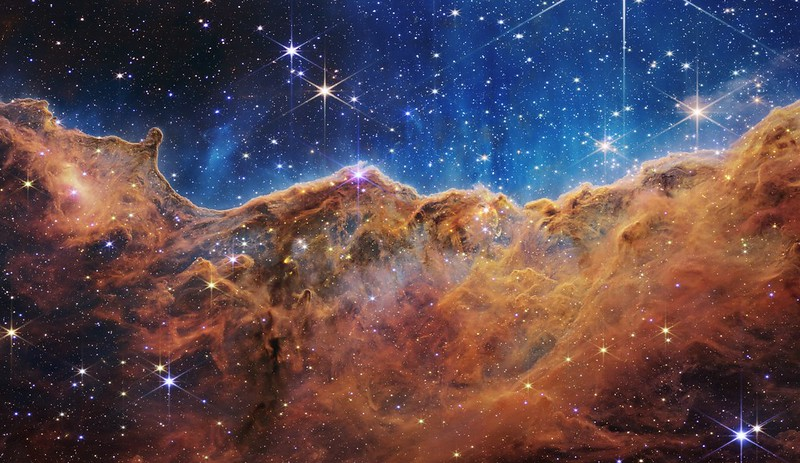
\includegraphics{james-webb-space-telescope-carina-nebula.jpg}
\end{center}

\noindent Photo credit: \href{https://webb.nasa.gov/}{James Webb Space Telescope}
(\href{https://www.flickr.com/photos/nasawebbtelescope/52259221868/in/album-72177720300469752/}{photo source})

\begin{abstract}
    \noindent This document provides an "explain like I'm five" explanation for three astronomy distance units:
    \noindent The astronomical unit (AU), the parsec, and the light-year. Refer to Table
    \noindent \ref{table:data} for the conversions between different distance units and meters.
\end{abstract}

\section*{Astronomical unit}  % Unnumbered section
The astronomical unit (AU) has traditionally been the average distance between the Sun and the
Earth, but has now been defined as exactly
\href{https://www.iau.org/static/resolutions/IAU2012_English.pdf}{149,597,870,700 m}.

\section*{Parsec}
To calculate the value of the parsec (pc), imagine you have a circle with a radius of 1 pc. Imagine
now that an arc length of 1 AU subtends an angle of 1" (1 second) at the center of this circle. What
this means is that, if you draw a straight line from one end of the 1 AU arc to the center of the
circle, and draw another line from the other end of the 1 AU arc to the center, then the angle
those two lines make is 1". \\

\noindent Note that there are 60 minutes in a circle, and there are 60 seconds in a minute, so 1"
is equal to \(\frac{1}{60 * 60}\) \textdegree. Converting to radians, 1" is equal to
\(\frac{\pi}{180 * 60 * 60}\) rad. \\

\noindent Also note that the formula for finding a length of arc in a circle is s = $\theta$r, with
$\theta$ being the angle in radians. This formula makes sense when you consider that the formula
for finding the circumference of a circle is C = 2$\pi$r. \\

\noindent Now, putting it all together, we can now solve for pc (the radius of the circle). Using
the arc length formula, AU = \(\frac{\pi pc}{180 * 60 * 60}\). Solving for pc, pc =
\(\frac{648000 AU}{\pi}\). Knowing that 1 AU = 149,597,870,700 m, 1 parsec is exactly
\(\frac{96,939,420,213,600,000}{\pi}\) m. \\

\noindent To learn more about how to derive the parsec, refer to
\href{https://www.nature.com/articles/s41567-019-0685-3}{this paper} or to the parsec's
\href{https://en.wikipedia.org/wiki/Parsec}{Wikipedia page}.

\section*{Light-year}
The light-year is the distance light travels in a year, with a year being defined as
\href{https://web.archive.org/web/20070216041250/http://www.iau.org/Units.234.0.html}{365.25 days}.
So, because the speed of light is defined as exactly 299,792,458 m/s, and there being 86,400 seconds
in a day, there is exactly 9,460,730,472,580,800 meters in a light-year.


\begin{table}[h!]
\centering
    \begin{tabular}{||c c||}
        \hline
        Distance unit & Meters \\ [0.5ex] 
        \hline\hline
        Astronomical unit & 149,597,870,700 \\
        \hline
        Parsec & \(\frac{96,939,420,213,600,000}{\pi}\) \\
        \hline
        Light-year & 9,460,730,472,580,800  \\
        \hline
        Gigameter & 1,000,000,000 \\ [1ex] 
        \hline
    \end{tabular}
\caption{Conversion to meters of astronomy distance units}
\label{table:data}

\end{table}

\end{document}
